% Created 2021-10-18 Mon 22:42
% Intended LaTeX compiler: xelatex
\documentclass[a4paper,12pt]{article}
\usepackage{graphicx}
\usepackage{grffile}
\usepackage{longtable}
\usepackage{wrapfig}
\usepackage{rotating}
\usepackage[normalem]{ulem}
\usepackage{amsmath}
\usepackage{textcomp}
\usepackage{amssymb}
\usepackage{capt-of}
\usepackage{hyperref}
\usepackage[margin=1.25in]{geometry}
\usepackage{fourier}
\usepackage{amsmath}
\usepackage[scaled]{helvet}
\linespread{1.10}
\setlength{\parindent}{0pt} %
\author{UINB Tech}
\date{2021}
\title{Fusotao Tokenomy Whitepaper\\\medskip
  \large v0.1.8\\\medskip
  \large https://www.fusotao.org}
\hypersetup{
 pdfauthor={UINB Tech,2021},
 pdftitle={Fusotao Economy Whitepaper},
 pdfkeywords={},
 pdfsubject={},
 pdfcreator={Emacs 27.2 (Org mode 9.5)}, 
 pdflang={English}}
\begin{document}

\maketitle
\clearpage

\section{About Fusotao}
\label{sec:1}
Fusotao is a completely decentralized and non-licensed protocol, including a series of general blockchain functions such as vote, staking, transfer, Token, virtual machine, and core modules for zero-knowledge proof validators, based on which can be developed decentralized financial products with high throughput and ultra-low transfer fees, while obtaining the transaction experience of centralized products. Zero-knowledge proof is the core of the entire project. In conjunction with the asset custody operation on the chain, the off-chain transaction system can realize matching transactions and proof of real transactions without the user's custody of assets. There is no artificial trust in the whole process.\\
To achieve the above-mentioned secure, fast, decentralized, and scalable Fuotao protocol, a complete set of Token economic incentive mechanism is needed to enable all participants in the ecosystem to jointly maintain the operation of the Fusatao system: on the one hand, the proportion of tokens and unlocking cycle need to be appropriately allocated to give full play to the initiative of project parties, developers, investors and community participants, Enable fusotao system to start smoothly and achieve long-term development; On the other hand, incentives need to be given to block packers, transaction certification service providers, transaction participants and community governance to achieve sufficient liquidity, security and stability of financial products on the chain.\\
TAO is the native token of the Fusotao protocol. It is the most important factor that motivates the properly function of Fusotao. It is also the proof of community participation in governance, development, transaction verification, and repurchase. \\
This section will describe TAO's economic model in detail.\\
\section{Tokenomy}
\label{sec:2}
Fusotao Token: TAO. Total Supply: $99,000,000$.\\
The allocation of the total supply of TAO is as follows:
\begin{itemize}
    \item $70\%$ or $69,300,000$ to the community, generated by the super node’s tenure as the time unit, each super node’s tenure lasts $1,339,200$ blocks ($93$ days), a total of 50 tenures, the total amount of TAO that can be generated during the t tenure: (Unit: $10000$ TAO)


\begin{equation*}
    curve(t)=\left\{\begin{matrix} -942t^2+6,000t+2,000,000, 0\leq t < 3 
        \\ 1,302,700, t = 3
\end{matrix}\right.
\end{equation*}
    Distribution methods of community rewards: 1. Transaction rewards (86\% of the total); 2. Community governance rewards (10\% of the total); 3. Zero-knowledge proof rewards (2\% of the total); 4. Mining Reward (2\% of total).

    \item $8\%$ or $7,920,000$ to Fusatao development, lockup for one year since the mainnet was launched and unlocked from the second year, linearly unlocked in 8 years and unlocked 1\% of the total tokens each year, unlocked by end of the ninth year.
    \item $8\%$ or $7,920,000$ to investors, including various rounds of personal and institutional investment and necessary public offerings. After the mainnet goes live, it requiring a lockup for 3 months and unlock 30\%, the remaining 70\% will be unlocked linearly in 12 months.
    \item $4\%$ or $3,960,000$ to the initial liquidity, it will all be used to provide initial liquidity (TAO/USDT) on centralized exchanges and decentralized exchanges after the mainnet goes live.
    \item $0.2\%$ or $198,000$ to Testnet incentive plan, used to reward early community users who participated in the testnet. It will be distributed after the mainnet goes live, and will be unlocked at a time after three months of lockup.
    \item $2.8\%$ or $2,772,000$ to market \& developer incentives. After the mainnet goes live, it will be linearly unlocked in 3 years, and $0.93\%$ will be unlocked every year.
    \item $2\%$ or $1,980,000$ to Community Airdrop, used to support community development after the mainnet goes live, airdrop to community users, and unlock immediately after the airdrop is completed.
    \item $5\%$ or $4,950,000$ to project development foundation, mainly used for long-term project development management, partner support, academic funding, public work, community development, etc. After the mainnet goes live, it will be unlocked linearly in 3 years.
\end{itemize}

\begin{figure}[htb]        
 \center{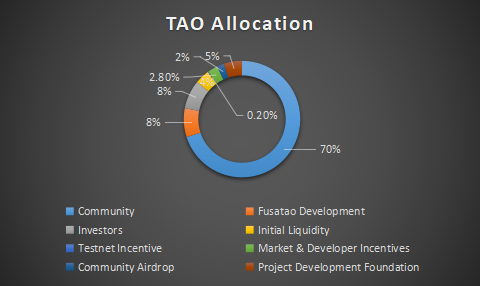
\includegraphics[width=11cm]  {1.png}}
 \caption{\label{1} TAO Allocation}      
\end{figure}

Fusotao is a completely decentralized and non-licensed community protocol, so most of the protocol tokens will be generated by community mining and distributed to communities that maintain protocol operations and participate in transactions. Community rewards accounted for 70\% of the total supply, of which transaction rewards accounted for 86\%, community governance rewards accounted for 10\%, block packaging rewards accounted for 2\%, and zero-knowledge proof rewards accounted for 2\%.\\
\begin{figure}[htb]        
 \center{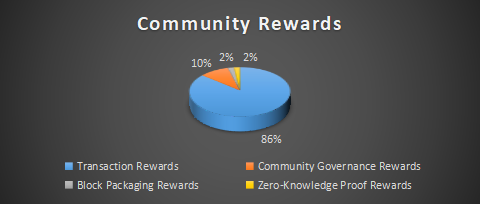
\includegraphics[width=11cm]  {2.png}}
 \caption{\label{2} Community Rewards}      
\end{figure}
Developers are important participants in the Fusotao protocol ecology and are responsible for building various infrastructure and maintenance protocols. The official development team will receive a total of 8\% of TAO Tokens within 9 years, some of which will be used for airdrops and incentives to participate in project testing and Community members of development.\\
4\% of the total amount of TAO will be live on the centralized and decentralized trading platform within 3 months of the mainnet goes live, providing initial liquidity of TAO.\\
In order to continue to grow the Fusotao community, we need a strong team composed of content producers, application developers, designers, coordinators, media, and consultants. TAO pass is a good way to motivate these participating teams, so we set up a project development foundation and set aside 5\% of TAO to allocate to these valuable contributors.\\
\section{TAO Token Unlock}
\label{sec:3}
We will be committed to the project technology upgrade and maintenance for a long time, and provide long-term incentives to community users. Tao Token is divided into 50 terms for approximately 13 years to unlock, and the development team's tokens are locked for one year and then linearly unlocked for 8 years. Starting from the mainnet goes live, the number of Tokens unlocked each year is as follows:\\

\begin{figure}[htb]        
 \center{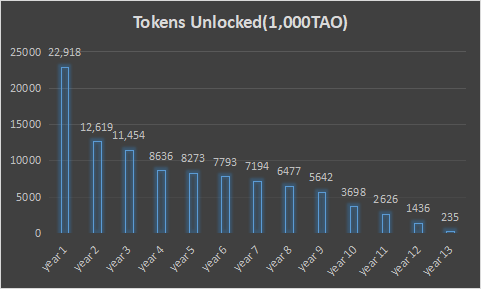
\includegraphics[width=11cm]  {3.png}}
 \caption{\label{3} Tokens unlocked each year}      
\end{figure}

Fusotao unlocks half of the tokens within 3 years after the mainnet goes live, and provides long-term incentives to the community in the following 10 years. The cumulative release curve of TAO is as follows:\\
\begin{figure}[htb]        
 \center{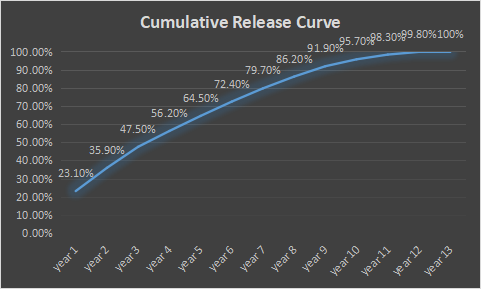
\includegraphics[width=11cm]  {4.png}}
 \caption{\label{4} The cumulative release curve of TAO}      
\end{figure}
\section{Community Rewards}
\label{sec:4}
It can be seen from the above-mentioned TAO Token system that 70\% of TAO Token will be allocated to “miners” participating in the community, that is, transaction users, community governance participants, block packagers, and zero-knowledge proof service providers. They are the main contributors to ensure the stable operation of the system and realize the fast and safe protocol.\\
$\operatorname{\mathbf{Trading reward:\ Proof-of-Trading (PoT)}}$\\
Fusotao is a completely decentralized protocol. The exchange developed above is a decentralized on-chain transaction, so there is no need to worry about problems with the exchange. Every transaction will receive TAO as a reward.\\
$\operatorname{\mathbf{Block Packing Reward:\ Proof-of-Block Packing (PoB)}}$\\
It is a common practice for blockchain projects to have token incentives for network nodes with packaging rights, which ensures the correct operation of the network. Super nodes are regularly voted by TAO holders and become block packaging nodes. They are rotated every 3 months. The total output of TAO during each term is determined by a specific quadratic curve.\\
$\operatorname{\mathbf{Community governance reward:\ Proof-of-Community Governance (PoC)}}$\\
If you do not want to run a super node on the chain alone, you can vote for others to become a super node. After the voted node is elected, you can continue to receive Tao rewards during the term of office.\\
$\operatorname{\mathbf{Zero-knowledge proof reward:\ Proof-of-ZK Snarks (PoZK)}}$\\
The Fusotao protocol is a verification protocol based on the order book matching model. Each transaction is verified on the chain before being cleared. PoZK will issue rewards in proportion to the transaction volume based on zero-knowledge proof contributed by users.\\
\section{Trading Rewards}
\label{sec:5}
$\mathbf{Overview}$\\
Trading rewards account for 86\% of community rewards and are the most important part of community rewards. Therefore, the trading reward rules are explained in detail here.\\
$\mathbf{Reward rules}$\\
The Fusotao protocol has a block time of 6s, and the transaction reward is distributed to all users who participate in the transaction of a specific transaction pair on the chain with $14,400$ blocks (24h) as the smallest unit. The TAO tokens that each trading user can obtain in a day will be determined by each user's cumulative transaction amount and TAO holdings as a percentage of the overall transaction amount and holdings. The specific calculation formula is as follows:\\
\begin{equation*}
    w=\left\{\begin{matrix} \sqrt{f \times t},t \ge 1 
        \\ \sqrt{f \times 1}, t < 1
\end{matrix}\right.
\end{equation*}

\begin{equation*}
    r=R \times \frac{w}{\sum_{i=0}^{n}w_{i}}
\end{equation*}
Notes:\\
\begin{itemize}
    \item $r$: The number of Token rewards obtained by personal transactions;
    \item $R$: The total number of token rewards distributed by all traders in the period;
    \item $f$: The accumulated amount of transactions by the trader during the period;
    \item $t$: The average number of TAO positions held by the trader during the period (measured once per block);
    \item $w$: Comprehensive weight of rewards for individual traders
    \item $\sum_{i=0}^{n}w_{i}$: The sum of the comprehensive weights of rewards for all traders;
    \item $n$: The total number of traders in the period.
\end{itemize}
$\mathbf{Reward \ collection \ time}$\\
After each time period (24h) ends, traders can apply for trading rewards.\\

\section{TAO Usage Scenarios}
\label{sec:6}
As Fusotao's native protocol Token, TAO not only represents the rights of the holder, but also has practical use value. TAO can be used in the following scenarios.\\
$\mathbf{Governance\ Token}$\\
Fusotao is a decentralized infrastructure with deep community participation and leadership. TAO is the only evidence for community participation in governance. TAO holders regularly vote to select super nodes with packaging rights from the nodes to ensure the correct operation of the network, and participate in voting and selection to obtain community governance rewards.\\
$\mathbf{Voting/staking\ to Create\ an\ Exchange}$\\
Fusotao is a completely non-licensed blockchain network. Any TAO holder can claim to be an exchange and provide transaction users with a matching certificate, and get rewards based on the proved transaction volume. Coin holders can initiate a proposal to create an exchange through the governance process, such as reaching a certain number of votes or obtaining a majority of votes to create their own exchange. For users who hold more coins, they can compete to create exchanges by staking TAO.\\
$\mathbf{Transaction\ Reward}$\\
Users who hold TAO and trade in an on-chain wallet can get rewards for proof of transaction volume.\\
$\mathbf{Repurchase\ and\ Destruction}$\\
The Fusotao agreement will charge a certain agreement fee as the gas fee for the transaction, and all the agreement fee will be used to repurchase TAO on a regular basis, and the TAO obtained will be directly destroyed.\\
$\mathbf{TAO\ Node\ Plan}$\\
Fusotao's block packaging rewards will be distributed to the elected super nodes, and holding more TAO tokens can campaign to become a super node.\\
\section{To\ Sum\ Up}
\label{sec:7}
TAO is the native token of the Fusotao protocol. It is an incentive link that encourages developers and the community to participate in building an ecosystem. More than 70\% of TAO Tokens will be rewarded to the community. Participating in transactions, community governance, block packaging, and providing zero-knowledge proof services can all be rewarded with TAO. Users who hold TAO can participate in Fustotao's ecological governance, vote or mortgage to create their own exchange, and pledge to become a super node with block packaging authority.\\
\end{document}
